\documentclass[11pt,t]{beamer}
\usetheme{kuleuven2}	%THEME OPTIONS for LOGO: kul (default), kulak, lrd,    ; OPTIONS for TITLE PAGE: normal (default), sedes


%%% OTHER SETTINGS
\usefonttheme[onlymath]{serif}			% math font with serifs, delete to make it sans-serif
\setbeamertemplate{footline}[frame number] 		% delete this line to remove footline bar on all frames
\usepackage[orientation=landscape,size=custom,width=16,height=9,scale=0.5,debug]{beamerposter} %enable for widescreen 16:9 ratio
%\titlegraphic{ \includegraphics[width=.2\paperwidth]{mytitlepagepic.png} } %optional title page image


%%% ADDED PACKAGES:
\usepackage[english]{babel}
\usepackage{amsfonts}
\usepackage{amssymb}
\usepackage{booktabs}
\usepackage[absolute,overlay]{textpos}
\usepackage{graphicx}
\usepackage{pgfplots}

\graphicspath{{../../Thesis/Images/} {graphics/}}

%%% TITLE PAGE INFO:
\title[Distributed Adversarial Attacks]{Evasive and efficient distributed adversarial attacks using PSO} %[]] will appear in footline
\subtitle{Intermediate presentation II}

\author{Sander Prenen}
\date{Mentors: I. Tsingenopoulos, V. Rimmer}
\institute{Thesis~supervisors:~Prof.~dr.~ir.~W.~Joosen,~Dr.~ir.~D.~Preuveneers}

\usepackage[backend=biber, style=verbose, defernumbers]{biblatex}
\addbibresource{citation.bib}
\setbeamertemplate{footnote}%
{%
  \parindent 1em\noindent%
  \raggedright\linespread{1}\selectfont%
  \hbox to 1.8em{\hfil\insertfootnotemark}\insertfootnotetext\par%
}
%\addtobeamertemplate{footnote}{}{\vspace{7ex}}

\begin{document}
\csname beamer@calculateheadfoot\endcsname %recalculate head and foot dimension

% Title page
\begin{frame}[plain,noframenumbering]
	\titlepage
\end{frame}

% Table of Contents
\begin{frame}{Outline}
	\hfill	{\large \parbox{.961\textwidth}{\tableofcontents[hideothersubsections]}}
\end{frame}

\section{Background}
\begin{frame}{Boundary attack\footcite{boundary_attack}}
\begin{figure}
\centering
\tikzset{every picture/.style={line width=0.75pt}} %set default line width to 0.75pt        
\begin{tikzpicture}[x=0.75pt,y=0.75pt,yscale=-0.8,xscale=0.8,every node/.style={scale=0.65}]
%uncomment if require: \path (0,300); %set diagram left start at 0, and has height of 300

%Shape: Polygon Curved [id:ds5185908380685693] 
\draw  [fill={rgb, 255:red, 155; green, 155; blue, 155 }  ,fill opacity=0.5 ] (77.12,91.56) .. controls (95.12,69.56) and (136.12,35.56) .. (170.12,73.56) .. controls (204.12,111.56) and (165.12,154.56) .. (194.12,183.56) .. controls (223.12,212.56) and (189.12,259.56) .. (159.12,263.56) .. controls (129.12,267.56) and (33.12,279.56) .. (30.12,246.56) .. controls (27.12,213.56) and (79.12,216.56) .. (90.12,178.56) .. controls (101.12,140.56) and (59.12,113.56) .. (77.12,91.56) -- cycle ;
%Shape: Star [id:dp7170747564600322] 
\draw  [fill={rgb, 255:red, 0; green, 0; blue, 0 }  ,fill opacity=1 ] (122.62,191.06) -- (124.83,195.53) -- (129.76,196.24) -- (126.19,199.72) -- (127.03,204.63) -- (122.62,202.31) -- (118.22,204.63) -- (119.06,199.72) -- (115.49,196.24) -- (120.42,195.53) -- cycle ;
%Shape: Star [id:dp10477759386916752] 
\draw  [fill={rgb, 255:red, 0; green, 0; blue, 0 }  ,fill opacity=1 ] (94.62,14.06) -- (96.83,18.53) -- (101.76,19.24) -- (98.19,22.72) -- (99.03,27.63) -- (94.62,25.31) -- (90.22,27.63) -- (91.06,22.72) -- (87.49,19.24) -- (92.42,18.53) -- cycle ;
%Straight Lines [id:da2531323347021954] 
\draw    (94.62,21.56) -- (101.19,66.01) ;
\draw [shift={(101.62,68.98)}, rotate = 261.6] [fill={rgb, 255:red, 0; green, 0; blue, 0 }  ][line width=0.08]  [draw opacity=0] (8.93,-4.29) -- (0,0) -- (8.93,4.29) -- cycle    ;
%Straight Lines [id:da6594852147606747] 
\draw    (101.79,68.14) -- (91.03,74.6) ;
\draw [shift={(88.46,76.14)}, rotate = 329.04] [fill={rgb, 255:red, 0; green, 0; blue, 0 }  ][line width=0.08]  [draw opacity=0] (8.93,-4.29) -- (0,0) -- (8.93,4.29) -- cycle    ;
%Straight Lines [id:da6002841525279263] 
\draw    (88.46,76.14) -- (80.11,85.56) ;
\draw [shift={(78.12,87.81)}, rotate = 311.53] [fill={rgb, 255:red, 0; green, 0; blue, 0 }  ][line width=0.08]  [draw opacity=0] (8.93,-4.29) -- (0,0) -- (8.93,4.29) -- cycle    ;
%Straight Lines [id:da9148455444041863] 
\draw    (78.12,87.81) -- (71.8,97.16) ;
\draw [shift={(70.12,99.64)}, rotate = 304.06] [fill={rgb, 255:red, 0; green, 0; blue, 0 }  ][line width=0.08]  [draw opacity=0] (8.93,-4.29) -- (0,0) -- (8.93,4.29) -- cycle    ;
%Straight Lines [id:da47669503735159546] 
\draw    (70.12,99.64) -- (71.42,110.17) ;
\draw [shift={(71.79,113.14)}, rotate = 262.96] [fill={rgb, 255:red, 0; green, 0; blue, 0 }  ][line width=0.08]  [draw opacity=0] (8.93,-4.29) -- (0,0) -- (8.93,4.29) -- cycle    ;
%Straight Lines [id:da26104674623686774] 
\draw    (71.79,113.14) -- (76.37,123.08) ;
\draw [shift={(77.62,125.81)}, rotate = 245.27] [fill={rgb, 255:red, 0; green, 0; blue, 0 }  ][line width=0.08]  [draw opacity=0] (8.93,-4.29) -- (0,0) -- (8.93,4.29) -- cycle    ;
%Straight Lines [id:da9792015265988265] 
\draw    (77.62,125.81) -- (82.31,135.45) ;
\draw [shift={(83.62,138.14)}, rotate = 244.06] [fill={rgb, 255:red, 0; green, 0; blue, 0 }  ][line width=0.08]  [draw opacity=0] (8.93,-4.29) -- (0,0) -- (8.93,4.29) -- cycle    ;
%Straight Lines [id:da8018833944649997] 
\draw    (83.62,138.14) -- (87.84,148.69) ;
\draw [shift={(88.96,151.48)}, rotate = 248.2] [fill={rgb, 255:red, 0; green, 0; blue, 0 }  ][line width=0.08]  [draw opacity=0] (8.93,-4.29) -- (0,0) -- (8.93,4.29) -- cycle    ;
%Straight Lines [id:da7469050329272713] 
\draw    (88.96,151.48) -- (90.55,163.17) ;
\draw [shift={(90.96,166.14)}, rotate = 262.23] [fill={rgb, 255:red, 0; green, 0; blue, 0 }  ][line width=0.08]  [draw opacity=0] (8.93,-4.29) -- (0,0) -- (8.93,4.29) -- cycle    ;
%Straight Lines [id:da36931886382540347] 
\draw    (90.96,166.14) -- (88.57,177.7) ;
\draw [shift={(87.96,180.64)}, rotate = 281.69] [fill={rgb, 255:red, 0; green, 0; blue, 0 }  ][line width=0.08]  [draw opacity=0] (8.93,-4.29) -- (0,0) -- (8.93,4.29) -- cycle    ;
%Straight Lines [id:da3125285737899821] 
\draw    (87.96,180.64) -- (83.39,189.01) ;
\draw [shift={(81.96,191.64)}, rotate = 298.61] [fill={rgb, 255:red, 0; green, 0; blue, 0 }  ][line width=0.08]  [draw opacity=0] (8.93,-4.29) -- (0,0) -- (8.93,4.29) -- cycle    ;

%Curve Lines [id:da7332610230112269] 
\draw    (243,111.62) .. controls (297.92,70.43) and (367.93,279.11) .. (405,99.26) ;
%Shape: Star [id:dp6998768571531213] 
\draw  [fill={rgb, 255:red, 0; green, 0; blue, 0 }  ,fill opacity=1 ] (322.11,170.74) -- (325.14,176.87) -- (331.9,177.85) -- (327.01,182.62) -- (328.16,189.36) -- (322.11,186.18) -- (316.06,189.36) -- (317.22,182.62) -- (312.32,177.85) -- (319.09,176.87) -- cycle ;
%Straight Lines [id:da9467918607674688] 
\draw    (299.68,128.68) -- (331.29,83.87) ;
\draw [shift={(333.02,81.42)}, rotate = 125.2] [fill={rgb, 255:red, 0; green, 0; blue, 0 }  ][line width=0.08]  [draw opacity=0] (8.93,-4.29) -- (0,0) -- (8.93,4.29) -- cycle    ;
%Shape: Ellipse [id:dp07084957668985581] 
\draw  [color={rgb, 255:red, 128; green, 128; blue, 128 }  ,draw opacity=1 ][dash pattern={on 4.5pt off 4.5pt}] (264.94,181.03) .. controls (264.94,149.46) and (290.54,123.86) .. (322.11,123.86) .. controls (353.69,123.86) and (379.28,149.46) .. (379.28,181.03) .. controls (379.28,212.61) and (353.69,238.2) .. (322.11,238.2) .. controls (290.54,238.2) and (264.94,212.61) .. (264.94,181.03) -- cycle ;
%Straight Lines [id:da7547924674466151] 
\draw    (299.68,128.68) -- (326.52,124.97) ;
\draw [shift={(329.49,124.56)}, rotate = 172.13] [fill={rgb, 255:red, 0; green, 0; blue, 0 }  ][line width=0.08]  [draw opacity=0] (8.93,-4.29) -- (0,0) -- (8.93,4.29) -- cycle    ;
%Straight Lines [id:da7777022216727221] 
\draw    (329.49,124.56) -- (326.01,147.88) ;
\draw [shift={(325.57,150.85)}, rotate = 278.49] [fill={rgb, 255:red, 0; green, 0; blue, 0 }  ][line width=0.08]  [draw opacity=0] (8.93,-4.29) -- (0,0) -- (8.93,4.29) -- cycle    ;
%Straight Lines [id:da931484330606797] 
\draw [color={rgb, 255:red, 128; green, 128; blue, 128 }  ,draw opacity=1 ] [dash pattern={on 0.84pt off 2.51pt}]  (333.02,81.42) -- (329.49,124.56) ;


% Text Node
\draw (328.21,263) node   [align=left] {\begin{minipage}[lt]{96.27pt}\setlength\topsep{0pt}
classified correctly
\end{minipage}};
% Text Node
\draw (326.21,62) node   [align=left] {\begin{minipage}[lt]{106.27pt}\setlength\topsep{0pt}
classified incorrectly
\end{minipage}};
% Text Node
\draw (325.12,211.56) node   [align=left] {\begin{minipage}[lt]{75pt}\setlength\topsep{0pt}
original image
\end{minipage}};
% Text Node
\draw (112.21,256.14) node   [align=left] {\begin{minipage}[lt]{96.27pt}\setlength\topsep{0pt}
classified correctly
\end{minipage}};
% Text Node
\draw (106,13) node [anchor=north west][inner sep=0.75pt]   [align=left] {starting image};
% Text Node
\draw (56.21,116) node  [rotate=-286.01] [align=left] {\begin{minipage}[lt]{106.27pt}\setlength\topsep{0pt}
classified incorrectly
\end{minipage}};
% Text Node
\draw (120.12,225.56) node   [align=left] {\begin{minipage}[lt]{75pt}\setlength\topsep{0pt}
original image
\end{minipage}};
% Text Node
\draw (381.43,114.71) node   [align=left] {\begin{minipage}[lt]{68pt}\setlength\topsep{0pt}
1
\end{minipage}};
% Text Node
\draw (377.9,148.85) node   [align=left] {\begin{minipage}[lt]{68pt}\setlength\topsep{0pt}
2
\end{minipage}};
% Text Node
\draw (330,130) node [anchor=north west][inner sep=0.75pt]   [align=left] {$\displaystyle \epsilon $};
% Text Node
\draw (305,86) node [anchor=north west][inner sep=0.75pt]   [align=left] {$\displaystyle \eta $};
\end{tikzpicture}
\end{figure}
\end{frame}

\begin{frame}{Biased boundary attack\footcite{brunner_guessing_2019}}
	\begin{itemize}
		\item Improvement on boundary attack
		\begin{itemize}
			\item Low frequency noise sampling
			\item Regional masking
			\item Gradients of surrogate models
		\end{itemize}
	\end{itemize}
	
	\begin{textblock*}{5cm}(9cm,1.5cm) % {block width} (coords)
		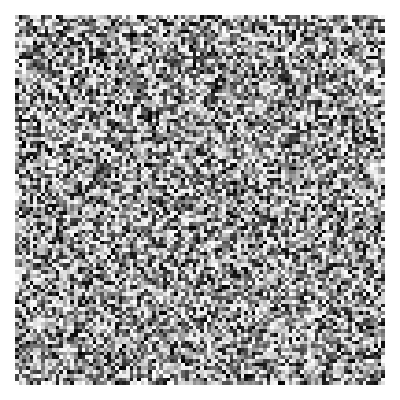
\includegraphics[scale=0.2]{gaussian_noise.png}
	\end{textblock*}
	\begin{textblock*}{5cm}(12cm,1.5cm) % {block width} (coords)
		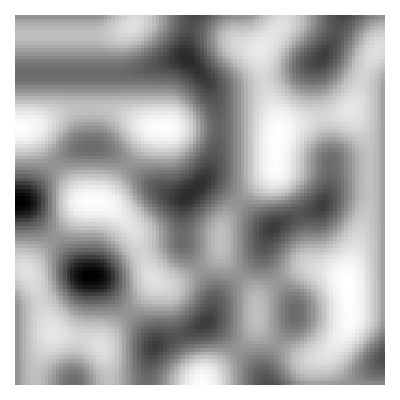
\includegraphics[scale=0.2]{perlin_noise.png}
	\end{textblock*}
\end{frame}

\begin{frame}{Stateful defense\footcite{chen_stateful_2019}}
	\centering
	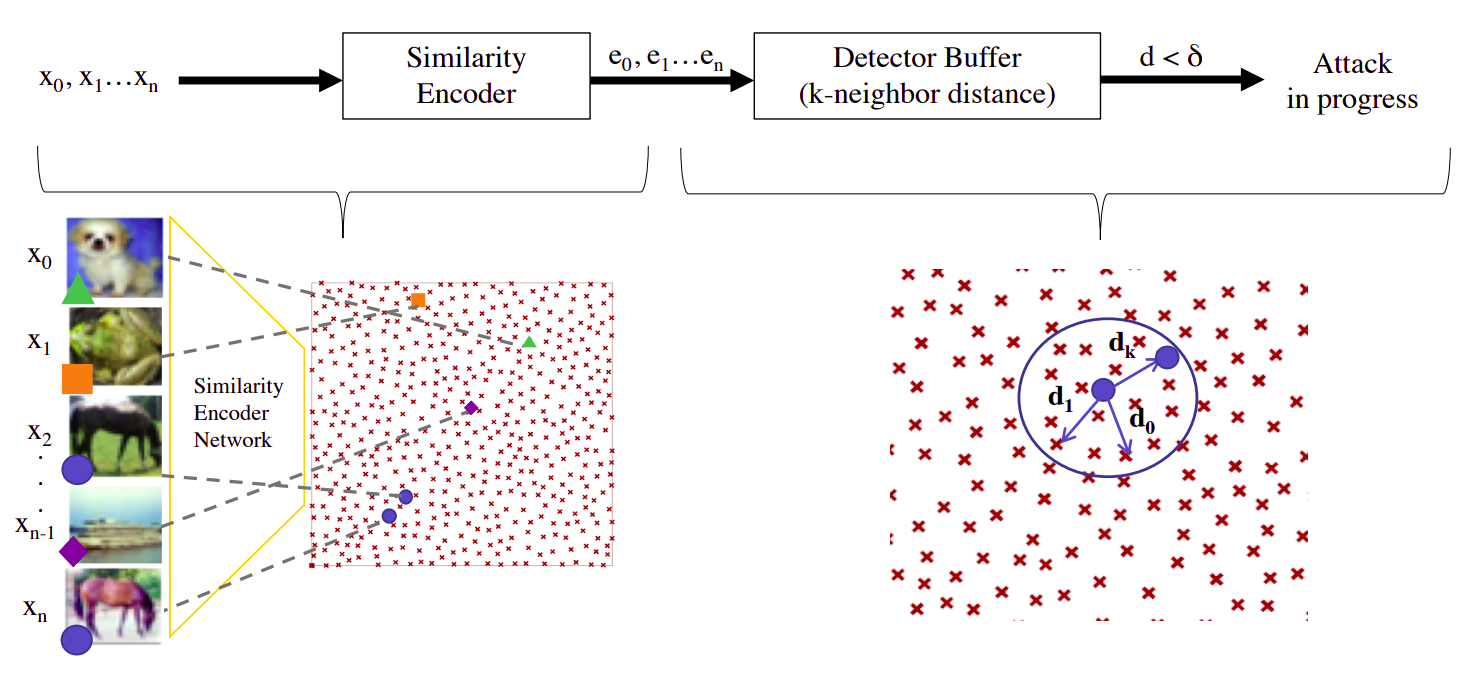
\includegraphics[width=0.8\textwidth]{stateful_detection.png}
\end{frame}

\begin{frame}{Particle swarm optimization}
	\begin{align*}
		v_{t} &= \underbrace{wv_{t-1}}_\text{Inertia} + \underbrace{c_pr_p(p_{t-1} - x_{t-1})}_\text{Individual best} + \underbrace{c_gr_g(g_{t-1} - x_{t-1})}_\text{Swarm best} \\
x_{t} &= x_{t-1} + v_{t} 
	\end{align*}

	\centering
\begin{tikzpicture}[x=0.75pt,y=0.75pt,yscale=-.7,xscale=.7,every node/.style={scale=0.7}]

%uncomment if require: \path (0,300); %set diagram left start at 0, and has height of 300

%Shape: Circle [id:dp06935534605548432] 
\draw  [fill={rgb, 255:red, 0; green, 0; blue, 0 }  ,fill opacity=1 ] (100,161) .. controls (100,152.16) and (107.16,145) .. (116,145) .. controls (124.84,145) and (132,152.16) .. (132,161) .. controls (132,169.84) and (124.84,177) .. (116,177) .. controls (107.16,177) and (100,169.84) .. (100,161) -- cycle ;
%Straight Lines [id:da36297070749556615] 
\draw [color={rgb, 255:red, 255; green, 0; blue, 0 }  ,draw opacity=1 ][line width=3]    (116,161) -- (109.44,250.02) ;
\draw [shift={(109,256)}, rotate = 274.21] [fill={rgb, 255:red, 255; green, 0; blue, 0 }  ,fill opacity=1 ][line width=0.08]  [draw opacity=0] (16.97,-8.15) -- (0,0) -- (16.97,8.15) -- cycle    ;
%Shape: Circle [id:dp2975589876543052] 
\draw  [fill={rgb, 255:red, 0; green, 0; blue, 0 }  ,fill opacity=1 ] (258,156) .. controls (258,147.16) and (265.16,140) .. (274,140) .. controls (282.84,140) and (290,147.16) .. (290,156) .. controls (290,164.84) and (282.84,172) .. (274,172) .. controls (265.16,172) and (258,164.84) .. (258,156) -- cycle ;
%Straight Lines [id:da11974704599725938] 
\draw [color={rgb, 255:red, 255; green, 0; blue, 0 }  ,draw opacity=1 ][line width=3]    (274,156) -- (267.44,245.02) ;
\draw [shift={(267,251)}, rotate = 274.21] [fill={rgb, 255:red, 255; green, 0; blue, 0 }  ,fill opacity=1 ][line width=0.08]  [draw opacity=0] (16.97,-8.15) -- (0,0) -- (16.97,8.15) -- cycle    ;
%Straight Lines [id:da34669530870861953] 
\draw [color={rgb, 255:red, 0; green, 0; blue, 255 }  ,draw opacity=1 ][line width=3]    (267,251) -- (207.74,176.69) ;
\draw [shift={(204,172)}, rotate = 51.43] [fill={rgb, 255:red, 0; green, 0; blue, 255 }  ,fill opacity=1 ][line width=0.08]  [draw opacity=0] (16.97,-8.15) -- (0,0) -- (16.97,8.15) -- cycle    ;
%Straight Lines [id:da2944239439562262] 
\draw [color={rgb, 255:red, 55; green, 158; blue, 54 }  ,draw opacity=1 ][line width=3]    (204,172) -- (217.97,148.18) ;
\draw [shift={(221,143)}, rotate = 120.38] [fill={rgb, 255:red, 55; green, 158; blue, 54 }  ,fill opacity=1 ][line width=0.08]  [draw opacity=0] (16.97,-8.15) -- (0,0) -- (16.97,8.15) -- cycle    ;
%Straight Lines [id:da9472051718664152] 
\draw [color={rgb, 255:red, 243; green, 0; blue, 255 }  ,draw opacity=1 ][line width=2.25]  [dash pattern={on 2.53pt off 3.02pt}]  (274,156) -- (224.88,143.95) ;
\draw [shift={(221,143)}, rotate = 13.78] [color={rgb, 255:red, 243; green, 0; blue, 255 }  ,draw opacity=1 ][line width=2.25]    (15.74,-7.06) .. controls (10.01,-3.31) and (4.76,-0.96) .. (0,0) .. controls (4.76,0.96) and (10.01,3.31) .. (15.74,7.06)   ;
%Straight Lines [id:da8503925276289086] 
\draw [color={rgb, 255:red, 0; green, 0; blue, 255 }  ,draw opacity=1 ][line width=3]    (116,161) -- (56.74,86.69) ;
\draw [shift={(53,82)}, rotate = 51.43] [fill={rgb, 255:red, 0; green, 0; blue, 255 }  ,fill opacity=1 ][line width=0.08]  [draw opacity=0] (16.97,-8.15) -- (0,0) -- (16.97,8.15) -- cycle    ;
%Straight Lines [id:da10251717157021911] 
\draw [color={rgb, 255:red, 55; green, 158; blue, 54 }  ,draw opacity=1 ][line width=3]    (116,161) -- (129.97,137.18) ;
\draw [shift={(133,132)}, rotate = 120.38] [fill={rgb, 255:red, 55; green, 158; blue, 54 }  ,fill opacity=1 ][line width=0.08]  [draw opacity=0] (16.97,-8.15) -- (0,0) -- (16.97,8.15) -- cycle    ;

% Text Node
\draw (46,156) node [anchor=north west][inner sep=0.75pt]   [align=left] {Particle};
% Text Node
\draw (115,244) node [anchor=north west][inner sep=0.75pt]   [align=left] {\textcolor[rgb]{1,0,0}{Inertia}};
% Text Node
\draw (38,65) node [anchor=north west][inner sep=0.75pt]  [color={rgb, 255:red, 0; green, 0; blue, 255 }  ,opacity=1 ] [align=left] {Swarm best};
% Text Node
\draw (94,110) node [anchor=north west][inner sep=0.75pt]  [color={rgb, 255:red, 55; green, 158; blue, 54 }  ,opacity=1 ] [align=left] {Individual best};
% Text Node
\draw (212,117) node [anchor=north west][inner sep=0.75pt]   [align=left] {\textcolor[rgb]{0.95,0,1}{New position}};
\end{tikzpicture}	
\end{frame}

\section{Research}
\begin{frame}{Goal}
	\begin{itemize}
		\item Propose new family of attacks
		\item Define threat model
		\item Experiment with the proposed attack
		\item Answer the following research questions:
		\begin{itemize}
			\item What are the (dis)advantages of using PSO in relation to vanilla adversarial attacks?
			\item How can PSO be combined with state of the art adversarial attacks?
			\item What are the (dis)advantages of distributing an adversarial attack?
		\end{itemize}
	\end{itemize}
\end{frame}

\section{Threat model}
\begin{frame}{Threat model}
	\begin{itemize}
		\item Decision based attack
		\item Targeted attack
		\item Stateful detection mechanism
		\begin{itemize}
			\item Query bounded buffer
			\item One buffer per account
		\end{itemize}
		\item Cost per account
		\item Cost per query
	\end{itemize}
\end{frame}

\section{Evaluation}
\begin{frame}{Evaluation protocol}
	\begin{itemize}
		\item MNIST\footcite{mnist} and CIFAR-10\footcite{cifar}
		\item Black box model\footcite{cw_attack}
	\end{itemize}
\end{frame}

\begin{frame}{Model architectures}
	\begin{table}
	\centering
    \begin{tabular}{lll}\toprule
        Layer type     & MNIST Model &CIFAR Model\\ \midrule
		Convolution + ReLU	&$3 \times 3 \times 32$ &$3\times3\times64$\\
		Convolution + ReLU	&$3 \times 3 \times 32$ &$3\times3\times64$\\
		Max Pooling					&$2 \times2$			&$2\times2$\\
		Convolution + ReLU	&$3 \times 3 \times 64$ &$3\times3\times128$\\
		Convolution + ReLU	&$3 \times 3 \times 64$ &$3\times3\times128$\\
		Max Pooling					&$2 \times2$			&$2\times2$\\
		Fully Connected + ReLU&$200	$				&$256$\\
		Fully Connected + ReLU&$200$					&$256$\\
		Softmax						&$10$						&$10$\\
        \bottomrule
    \end{tabular}
    \label{tbl:architectures}
\end{table}
\end{frame}

\begin{frame}{Evaluation protocol}
	\begin{itemize}
		\item MNIST and CIFAR-10
		\item Black box model
		\item List of experiments
		\begin{itemize}
			\item Original image (+label)
			\item Target label
			\item Starting position(s)
		\end{itemize}
		\item Query bounded detector buffer of size 1000
		\item Number of neighbors is 50
		\item Query budget of 25000
	\end{itemize}
\end{frame}

\begin{frame}{Baseline results}
	\begin{itemize}
		\item Determine baseline distance ($L_2$) and number of detections for biased boundary attack
		\item Hyperparameters as suggested in original paper\footcite{brunner_guessing_2019}
	\end{itemize}
	\begin{table}
	\centering
	\begin{tabular}{lrrrr}\toprule
			& \multicolumn{2}{c}{MNIST} &\multicolumn{2}{c}{CIFAR} \\ \cmidrule(r){2-3} \cmidrule(r){4-5}
	Attack				&Distance	&Detections	&Distance	&Detections \\ \midrule
	Baseline BBA	&3.027		&339		&1.359			&475 \\ \bottomrule
	
	\end{tabular}
	\end{table}
\end{frame}

\begin{frame}{Combining BBA and PSO}
	\centering
	\begin{tikzpicture}[x=0.75pt,y=0.75pt,yscale=-.8,xscale=.8, every node/.style={scale=0.8}]
%uncomment if require: \path (0,300); %set diagram left start at 0, and has height of 300

%Shape: Polygon Curved [id:ds39418321723754923] 
\draw  [fill={rgb, 255:red, 155; green, 155; blue, 155 }  ,fill opacity=0.5 ] (365.12,90.5) .. controls (383.12,68.5) and (424.12,34.5) .. (458.12,72.5) .. controls (492.12,110.5) and (453.12,153.5) .. (482.12,182.5) .. controls (511.12,211.5) and (477.12,258.5) .. (447.12,262.5) .. controls (417.12,266.5) and (321.12,278.5) .. (318.12,245.5) .. controls (315.12,212.5) and (367.12,215.5) .. (378.12,177.5) .. controls (389.12,139.5) and (347.12,112.5) .. (365.12,90.5) -- cycle ;
%Shape: Star [id:dp17995230177708343] 
\draw  [fill={rgb, 255:red, 0; green, 0; blue, 0 }  ,fill opacity=1 ] (410.62,190) -- (412.83,194.47) -- (417.76,195.18) -- (414.19,198.66) -- (415.03,203.57) -- (410.62,201.25) -- (406.22,203.57) -- (407.06,198.66) -- (403.49,195.18) -- (408.42,194.47) -- cycle ;
%Shape: Star [id:dp263511542953333] 
\draw  [fill={rgb, 255:red, 0; green, 0; blue, 0 }  ,fill opacity=1 ] (382.62,13) -- (384.83,17.47) -- (389.76,18.18) -- (386.19,21.66) -- (387.03,26.57) -- (382.62,24.25) -- (378.22,26.57) -- (379.06,21.66) -- (375.49,18.18) -- (380.42,17.47) -- cycle ;
%Straight Lines [id:da12241666866362477] 
\draw    (382.62,20.5) -- (389.19,64.95) ;
\draw [shift={(389.62,67.92)}, rotate = 261.6] [fill={rgb, 255:red, 0; green, 0; blue, 0 }  ][line width=0.08]  [draw opacity=0] (8.93,-4.29) -- (0,0) -- (8.93,4.29) -- cycle    ;
%Straight Lines [id:da7985170559413728] 
\draw    (389.79,67.08) -- (379.03,73.54) ;
\draw [shift={(376.46,75.08)}, rotate = 329.04] [fill={rgb, 255:red, 0; green, 0; blue, 0 }  ][line width=0.08]  [draw opacity=0] (8.93,-4.29) -- (0,0) -- (8.93,4.29) -- cycle    ;
%Straight Lines [id:da5286207592270582] 
\draw    (376.46,75.08) -- (368.11,84.5) ;
\draw [shift={(366.12,86.75)}, rotate = 311.53] [fill={rgb, 255:red, 0; green, 0; blue, 0 }  ][line width=0.08]  [draw opacity=0] (8.93,-4.29) -- (0,0) -- (8.93,4.29) -- cycle    ;
%Straight Lines [id:da4098354744836743] 
\draw    (366.12,86.75) -- (359.8,96.1) ;
\draw [shift={(358.12,98.58)}, rotate = 304.06] [fill={rgb, 255:red, 0; green, 0; blue, 0 }  ][line width=0.08]  [draw opacity=0] (8.93,-4.29) -- (0,0) -- (8.93,4.29) -- cycle    ;
%Straight Lines [id:da7402027038712158] 
\draw    (358.12,98.58) -- (359.42,109.11) ;
\draw [shift={(359.79,112.08)}, rotate = 262.96] [fill={rgb, 255:red, 0; green, 0; blue, 0 }  ][line width=0.08]  [draw opacity=0] (8.93,-4.29) -- (0,0) -- (8.93,4.29) -- cycle    ;
%Straight Lines [id:da22742294505428506] 
\draw    (359.79,112.08) -- (364.37,122.03) ;
\draw [shift={(365.62,124.75)}, rotate = 245.27] [fill={rgb, 255:red, 0; green, 0; blue, 0 }  ][line width=0.08]  [draw opacity=0] (8.93,-4.29) -- (0,0) -- (8.93,4.29) -- cycle    ;
%Shape: Boxed Line [id:dp17555971988752717] 
\draw    (362.2,200.74) -- (368.55,193.64) ;
\draw [shift={(370.55,191.4)}, rotate = 131.8] [fill={rgb, 255:red, 0; green, 0; blue, 0 }  ][line width=0.08]  [draw opacity=0] (8.93,-4.29) -- (0,0) -- (8.93,4.29) -- cycle    ;
%Shape: Star [id:dp5469311004467188] 
\draw  [fill={rgb, 255:red, 0; green, 0; blue, 0 }  ,fill opacity=1 ] (533.42,103.8) -- (535.63,108.27) -- (540.56,108.98) -- (536.99,112.46) -- (537.83,117.37) -- (533.42,115.05) -- (529.02,117.37) -- (529.86,112.46) -- (526.29,108.98) -- (531.22,108.27) -- cycle ;
%Shape: Star [id:dp8199494411723183] 
\draw  [fill={rgb, 255:red, 0; green, 0; blue, 0 }  ,fill opacity=1 ] (525,239.51) -- (527.2,243.97) -- (532.13,244.69) -- (528.57,248.17) -- (529.41,253.07) -- (525,250.76) -- (520.59,253.07) -- (521.43,248.17) -- (517.87,244.69) -- (522.8,243.97) -- cycle ;
%Shape: Star [id:dp3621439940158031] 
\draw  [fill={rgb, 255:red, 0; green, 0; blue, 0 }  ,fill opacity=1 ] (324.22,281.14) -- (326.43,285.61) -- (331.36,286.32) -- (327.79,289.8) -- (328.63,294.71) -- (324.22,292.39) -- (319.82,294.71) -- (320.66,289.8) -- (317.09,286.32) -- (322.02,285.61) -- cycle ;
%Shape: Star [id:dp886425904787334] 
\draw  [fill={rgb, 255:red, 0; green, 0; blue, 0 }  ,fill opacity=1 ] (298.22,198.74) -- (300.43,203.21) -- (305.36,203.92) -- (301.79,207.4) -- (302.63,212.31) -- (298.22,209.99) -- (293.82,212.31) -- (294.66,207.4) -- (291.09,203.92) -- (296.02,203.21) -- cycle ;
%Straight Lines [id:da29737150039250193] 
\draw    (533.42,111.3) -- (473.43,154.98) ;
\draw [shift={(471,156.74)}, rotate = 323.95] [fill={rgb, 255:red, 0; green, 0; blue, 0 }  ][line width=0.08]  [draw opacity=0] (8.93,-4.29) -- (0,0) -- (8.93,4.29) -- cycle    ;
%Straight Lines [id:da564242749820822] 
\draw    (298.22,206.24) -- (359.21,201) ;
\draw [shift={(362.2,200.74)}, rotate = 175.09] [fill={rgb, 255:red, 0; green, 0; blue, 0 }  ][line width=0.08]  [draw opacity=0] (8.93,-4.29) -- (0,0) -- (8.93,4.29) -- cycle    ;
%Straight Lines [id:da8824188996602935] 
\draw    (525,247.01) -- (490.26,231.18) ;
\draw [shift={(487.53,229.94)}, rotate = 24.49] [fill={rgb, 255:red, 0; green, 0; blue, 0 }  ][line width=0.08]  [draw opacity=0] (8.93,-4.29) -- (0,0) -- (8.93,4.29) -- cycle    ;
%Straight Lines [id:da172043009485096] 
\draw    (324.22,288.64) -- (343.77,267.35) ;
\draw [shift={(345.8,265.14)}, rotate = 132.55] [fill={rgb, 255:red, 0; green, 0; blue, 0 }  ][line width=0.08]  [draw opacity=0] (8.93,-4.29) -- (0,0) -- (8.93,4.29) -- cycle    ;
%Shape: Boxed Line [id:dp5913488094519332] 
\draw    (370.55,191.4) -- (374.75,182.84) ;
\draw [shift={(376.07,180.15)}, rotate = 116.11] [fill={rgb, 255:red, 0; green, 0; blue, 0 }  ][line width=0.08]  [draw opacity=0] (8.93,-4.29) -- (0,0) -- (8.93,4.29) -- cycle    ;
%Shape: Boxed Line [id:dp8616221435272089] 
\draw    (487.53,229.94) -- (491.55,221.3) ;
\draw [shift={(492.81,218.58)}, rotate = 114.93] [fill={rgb, 255:red, 0; green, 0; blue, 0 }  ][line width=0.08]  [draw opacity=0] (8.93,-4.29) -- (0,0) -- (8.93,4.29) -- cycle    ;
%Shape: Boxed Line [id:dp5796326247856174] 
\draw    (492.81,218.58) -- (494.7,209.24) ;
\draw [shift={(495.29,206.29)}, rotate = 101.39] [fill={rgb, 255:red, 0; green, 0; blue, 0 }  ][line width=0.08]  [draw opacity=0] (8.93,-4.29) -- (0,0) -- (8.93,4.29) -- cycle    ;
%Shape: Boxed Line [id:dp044334919963415986] 
\draw    (495.29,206.29) -- (492.57,197.16) ;
\draw [shift={(491.71,194.29)}, rotate = 73.42] [fill={rgb, 255:red, 0; green, 0; blue, 0 }  ][line width=0.08]  [draw opacity=0] (8.93,-4.29) -- (0,0) -- (8.93,4.29) -- cycle    ;
%Shape: Boxed Line [id:dp4387546700476397] 
\draw    (491.71,194.29) -- (486.61,186.24) ;
\draw [shift={(485,183.71)}, rotate = 57.58] [fill={rgb, 255:red, 0; green, 0; blue, 0 }  ][line width=0.08]  [draw opacity=0] (8.93,-4.29) -- (0,0) -- (8.93,4.29) -- cycle    ;
%Shape: Boxed Line [id:dp8947094222533136] 
\draw    (485,183.71) -- (478.98,176.32) ;
\draw [shift={(477.09,173.99)}, rotate = 50.85] [fill={rgb, 255:red, 0; green, 0; blue, 0 }  ][line width=0.08]  [draw opacity=0] (8.93,-4.29) -- (0,0) -- (8.93,4.29) -- cycle    ;
%Shape: Boxed Line [id:dp8126738394252795] 
\draw    (471,156.74) -- (473.27,166) ;
\draw [shift={(473.99,168.91)}, rotate = 256.19] [fill={rgb, 255:red, 0; green, 0; blue, 0 }  ][line width=0.08]  [draw opacity=0] (8.93,-4.29) -- (0,0) -- (8.93,4.29) -- cycle    ;
%Shape: Boxed Line [id:dp14754319972001273] 
\draw    (345.8,265.14) -- (355.11,267.18) ;
\draw [shift={(358.04,267.82)}, rotate = 192.33] [fill={rgb, 255:red, 0; green, 0; blue, 0 }  ][line width=0.08]  [draw opacity=0] (8.93,-4.29) -- (0,0) -- (8.93,4.29) -- cycle    ;
%Shape: Boxed Line [id:dp8374639915608668] 
\draw    (358.04,267.82) -- (367.46,269.26) ;
\draw [shift={(370.43,269.71)}, rotate = 188.71] [fill={rgb, 255:red, 0; green, 0; blue, 0 }  ][line width=0.08]  [draw opacity=0] (8.93,-4.29) -- (0,0) -- (8.93,4.29) -- cycle    ;
%Shape: Boxed Line [id:dp496623104677657] 
\draw    (370.43,269.71) -- (379.95,269.39) ;
\draw [shift={(382.95,269.29)}, rotate = 178.04] [fill={rgb, 255:red, 0; green, 0; blue, 0 }  ][line width=0.08]  [draw opacity=0] (8.93,-4.29) -- (0,0) -- (8.93,4.29) -- cycle    ;
%Shape: Boxed Line [id:dp34473561543285314] 
\draw    (382.95,269.29) -- (392.47,268.77) ;
\draw [shift={(395.46,268.61)}, rotate = 176.92] [fill={rgb, 255:red, 0; green, 0; blue, 0 }  ][line width=0.08]  [draw opacity=0] (8.93,-4.29) -- (0,0) -- (8.93,4.29) -- cycle    ;
%Shape: Boxed Line [id:dp22829712791209555] 
\draw    (395.46,268.61) -- (404.98,268.23) ;
\draw [shift={(407.98,268.11)}, rotate = 177.71] [fill={rgb, 255:red, 0; green, 0; blue, 0 }  ][line width=0.08]  [draw opacity=0] (8.93,-4.29) -- (0,0) -- (8.93,4.29) -- cycle    ;

%Shape: Polygon Curved [id:ds013419098702227128] 
\draw  [fill={rgb, 255:red, 155; green, 155; blue, 155 }  ,fill opacity=0.5 ] (72.05,88.7) .. controls (90.05,66.7) and (131.05,32.7) .. (165.05,70.7) .. controls (199.05,108.7) and (160.05,151.7) .. (189.05,180.7) .. controls (218.05,209.7) and (184.05,256.7) .. (154.05,260.7) .. controls (124.05,264.7) and (28.05,276.7) .. (25.05,243.7) .. controls (22.05,210.7) and (74.05,213.7) .. (85.05,175.7) .. controls (96.05,137.7) and (54.05,110.7) .. (72.05,88.7) -- cycle ;
%Shape: Star [id:dp9534459695500062] 
\draw  [fill={rgb, 255:red, 0; green, 0; blue, 0 }  ,fill opacity=1 ] (117.55,188.2) -- (119.76,192.67) -- (124.68,193.38) -- (121.12,196.86) -- (121.96,201.77) -- (117.55,199.45) -- (113.14,201.77) -- (113.99,196.86) -- (110.42,193.38) -- (115.35,192.67) -- cycle ;
%Shape: Star [id:dp3150974101447812] 
\draw  [fill={rgb, 255:red, 0; green, 0; blue, 0 }  ,fill opacity=1 ] (231.93,237.71) -- (234.13,242.17) -- (239.06,242.89) -- (235.49,246.37) -- (236.34,251.28) -- (231.93,248.96) -- (227.52,251.28) -- (228.36,246.37) -- (224.79,242.89) -- (229.72,242.17) -- cycle ;
%Straight Lines [id:da8721626382201679] 
\draw    (231.93,245.21) -- (197.19,229.38) ;
\draw [shift={(194.46,228.14)}, rotate = 24.49] [fill={rgb, 255:red, 0; green, 0; blue, 0 }  ][line width=0.08]  [draw opacity=0] (8.93,-4.29) -- (0,0) -- (8.93,4.29) -- cycle    ;
%Shape: Boxed Line [id:dp35233924811215767] 
\draw    (194.46,228.14) -- (198.48,219.5) ;
\draw [shift={(199.74,216.78)}, rotate = 114.93] [fill={rgb, 255:red, 0; green, 0; blue, 0 }  ][line width=0.08]  [draw opacity=0] (8.93,-4.29) -- (0,0) -- (8.93,4.29) -- cycle    ;
%Shape: Boxed Line [id:dp47377705399021885] 
\draw    (199.74,216.78) -- (201.62,207.44) ;
\draw [shift={(202.22,204.5)}, rotate = 101.39] [fill={rgb, 255:red, 0; green, 0; blue, 0 }  ][line width=0.08]  [draw opacity=0] (8.93,-4.29) -- (0,0) -- (8.93,4.29) -- cycle    ;
%Shape: Boxed Line [id:dp01327277725498055] 
\draw    (202.22,204.5) -- (199.5,195.36) ;
\draw [shift={(198.64,192.49)}, rotate = 73.42] [fill={rgb, 255:red, 0; green, 0; blue, 0 }  ][line width=0.08]  [draw opacity=0] (8.93,-4.29) -- (0,0) -- (8.93,4.29) -- cycle    ;
%Shape: Boxed Line [id:dp6860848467619505] 
\draw    (198.64,192.49) -- (193.53,184.44) ;
\draw [shift={(191.92,181.91)}, rotate = 57.58] [fill={rgb, 255:red, 0; green, 0; blue, 0 }  ][line width=0.08]  [draw opacity=0] (8.93,-4.29) -- (0,0) -- (8.93,4.29) -- cycle    ;
%Shape: Boxed Line [id:dp2849658598230065] 
\draw    (191.92,181.91) -- (185.91,174.52) ;
\draw [shift={(184.01,172.19)}, rotate = 50.85] [fill={rgb, 255:red, 0; green, 0; blue, 0 }  ][line width=0.08]  [draw opacity=0] (8.93,-4.29) -- (0,0) -- (8.93,4.29) -- cycle    ;


% Text Node
\draw (107.14,250.13) node   [align=left] {\begin{minipage}[lt]{96.27pt}\setlength\topsep{0pt}
classified correctly
\end{minipage}};
% Text Node
\draw (51.61,113.14) node  [rotate=-286.01] [align=left] {\begin{minipage}[lt]{106.27pt}\setlength\topsep{0pt}
classified incorrectly
\end{minipage}};
% Text Node
\draw (119.05,223.33) node   [align=left] {\begin{minipage}[lt]{75pt}\setlength\topsep{0pt}
original image
\end{minipage}};
% Text Node
\draw (400.21,251.93) node   [align=left] {\begin{minipage}[lt]{96.27pt}\setlength\topsep{0pt}
classified correctly
\end{minipage}};
% Text Node
\draw (344.71,114.94) node  [rotate=-286.01] [align=left] {\begin{minipage}[lt]{106.27pt}\setlength\topsep{0pt}
classified incorrectly
\end{minipage}};
% Text Node
\draw (412.12,225.13) node   [align=left] {\begin{minipage}[lt]{75pt}\setlength\topsep{0pt}
original image
\end{minipage}};
\end{tikzpicture}
\end{frame}

\begin{frame}{Combining BBA and PSO}
	\begin{itemize}
		\item Multiple starting positions
		\item More aggressive
		\item Communication between particles
		\item Fitness function
	\end{itemize}
	\begin{align*}
	f(x) = 
	\begin{cases}
 		\| x - x^\prime\|_2,	&\text{if } x \text{ is adversarial}\\
 		+\infty, 		& \text{else}
	\end{cases}
\end{align*}
\end{frame}

\begin{frame}{Combining BBA and PSO}
	\begin{table}
	\centering
	\begin{tabular}{lrrrr}\toprule
			& \multicolumn{2}{c}{MNIST} &\multicolumn{2}{c}{CIFAR} \\ \cmidrule(r){2-3} \cmidrule(r){4-5}
	Attack				&Distance	&Detections	&Distance	&Detections \\ \midrule
	Baseline BBA	&3.027		&339		&1.359			&475 \\
	PSO-BBA (5 particles)	&2.691			&173			&1.133				&301 \\ 
	PSO-BBA (10 particles)	&2.788			&107			&1.782				&243 \\
	\bottomrule
	\end{tabular}
\end{table}
\end{frame}

\begin{frame}{Combining BBA and PSO}
	\begin{itemize}
		\item Detections happen at the end of attack
	\end{itemize}
	\vfill
	\centering
	\begin{tikzpicture}
\begin{axis}[width=12cm, height=5cm, xmin=0,xmax=25000, xlabel=Calls, ylabel=Detections, tick label style={/pgf/number format/fixed}, scaled ticks=false, enlarge x limits=0.01, xtick={0,5000,10000,15000,20000,25000},legend pos=north west,	legend style={draw=none},]
\addplot table[col sep=comma,x index=1,y expr=\thisrowno{0} + 1,mark=none] {../../Thesis/Data/detections_bba.csv};
\addlegendentry{BBA};
\addplot table[col sep=comma,x index=1,y expr=\thisrowno{0} + 1,mark=none] {../../Thesis/Data/detections_pso_bba.csv};
\addlegendentry{PSO-BBA};
\end{axis};
\end{tikzpicture}
\end{frame}

\begin{frame}{Distributing the query submission}
	\vfill
	\centering
\begin{tikzpicture}
\begin{scope}[every node/.style={rectangle,thick,draw,anchor=base, minimum width=20mm}]
	\node[align=center] (N1) at (3,5) {Node 1};
	\node[align=center] (N2) at (3,4) {Node 2};
	\node[align=center] (N3) at (3,3) {Node 3};
	\node[align=center] (NN) at (3,1) {Node $N$};
\end{scope}

\node[align=center,anchor=base, minimum width=20mm,rectangle] (N) at (3,2) {$\ldots$};

\begin{scope}[every node/.style={rectangle,thick,draw,anchor=base,minimum width=20mm, minimum height=10mm}]
	\node[align=right, left= 35mm of N3] (A) {Algorithm};
	\node[align=left, right= 35mm of N3] (M) {Model};
\end{scope}

\begin{scope}[]
	\path [->] (A.east) edge (N1.west);
	\path [->] (A.east) edge (N2.west);
	\path [->] (A.east) edge (N3.west);
%	\path [->] (A.east) edge (N.west);
	\path [->] (A.east) edge (NN.west);

	\path [->] (N1.east) edge (M.west);
	\path [->] (N2.east) edge (M.west);
	\path [->] (N3.east) edge (M.west);
%	\path [->] (N.east) edge (M.west);
	\path [->] (NN.east) edge (M.west);	
\end{scope}
\end{tikzpicture}
\end{frame}

\begin{frame}{Distributing the query submission}

\end{frame}

\end{document}